% Provenance (never printed): old terminale S material on the disappearance of
% mountain ranges (erosion, transport, sedimentation, isostatic rebound, the
% recycling of continental material). Owner (Sync 0/1): denudation rate,
% sediment load (bed, suspended, dissolved), isostatic rebound, detrital rock,
% diagenesis. Weathering, erosion, deposition are Book 1's (g5); hydrolysis and
% clay minerals g10.07's; discharge g10.08's; isostasy and Airy's model g11.03's;
% sedimentary basin g11.09's; mountain root g12.01's; metamorphism g12.03's;
% half-life is physics' (recalled in prose). Figures: figdata/grade-12/relief_decay.py
% (rates, decay curves, the Varden unconformity from figdata/shared/region.py).
\chapter{山脉的消亡}\label{ch:g12:destruction-of-mountains}

从国际空间站望去，北美东部的阿巴拉契亚山脉
呈现出一幅醒目的图景：一道道狭长、色暗、覆盖森林的山脊
与浅色的耕作山谷相间，照片所示范围内绵延超过 \qty{500}{km}，
见下图。山脊由坚硬的岩层构成，它们在非洲向北美洲挤压时被揉成紧密\omterm{def:g12:mountain-building:fold}{褶皱}，
发生于石炭纪和二叠纪，
距今超过 2.5 亿年。如今，其最高峰米切尔山，
是密西西比河以东的最高点，高出海平面
\qty{2037}{m}，不到珠穆朗玛峰高度的四分之一。
% ledger: photo:g12-appalachians, usgs:alleghanian, usgs:alleghanian-age, ics:base.Triassic, ncparks:mitchell (6684 ft), tht:everest (Book 1 row, 8848.86 m)

\begin{omfigure}
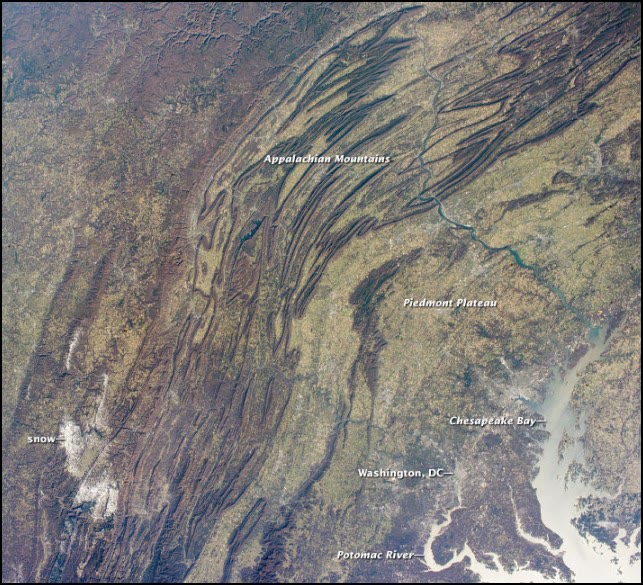
\includegraphics[width=0.6\linewidth]{images/book2/g12-iss-appalachians.jpg}

{\small 山脊与山谷相间的阿巴拉契亚山脉，从宾夕法尼亚州东北部
（右上角）延伸至西弗吉尼亚州，由国际空间站拍摄，
拍摄于 2012 年 11 月 17 日。覆林的山脊由坚硬的岩层构成，
耕作的山谷则由较软的岩层构成。照片：NASA（公有领域）。}
\end{omfigure}
% ledger: photo:g12-appalachians

山脉并不会长存。自隆起之时起，雨水、冰川和河流便开始侵蚀它；
被搬运走的岩石最终汇入大海，并在那里变为新的岩石。
本章测算这一过程的快慢，追踪碎屑
被搬运到其固结成岩的地方，并说明
一座正被剥蚀的山脉为何仍会持续抬升。

\begin{recall}
风化使岩石在原地破碎；侵蚀将碎屑搬走，
沉积则将其堆积到别处（第 1 册，五年级）。\omterm{def:g10:soil-formation:chemical-weathering}{化学风化}
通过\omterm{def:g10:soil-formation:hydrolysis}{水解}将长石转变为\omterm{def:g10:soil-formation:clay}{黏土矿物}
（见\cref{ch:g10:soil-formation}）。河流的\omterm{def:g10:drainage-basins:discharge}{流量}是指
单位时间内流经某一点的水体体积（见\cref{ch:g10:drainage-basins}）。
地壳依\omterm{def:g11:lithosphere-asthenosphere:isostasy}{地壳均衡}原理漂浮于地幔之上；按艾里模型，地壳
增厚 $\Delta H$ 的区域，会高出 $\Delta H\,(\rho_m - \rho_c)/\rho_m$
（见\cref{ch:g11:lithosphere-asthenosphere}），而高山则
由厚地壳形成的\omterm{def:g12:continental-crust:root}{山根}支撑（见\cref{ch:g12:continental-crust}）。沉积物堆积于
\omterm{def:g11:fossil-fuel-geology:basin}{沉积盆地}中（见\cref{ch:g11:fossil-fuel-geology}）。埋藏于
造山带深处的岩石会发生变质（见\cref{ch:g12:metamorphic-rocks}）。
\end{recall}

\section{陆地被剥蚀的速度有多快？}

\begin{definition}[剥蚀速率]\label{def:g12:destruction-of-mountains:denudation}
某区域的\emph{剥蚀速率}\index{剥蚀速率}是指
风化与侵蚀在单位时间内共同移去的岩石平均厚度。
通常以每百万年多少米表示，
（\unit{m/Ma}），这与每千年多少毫米相同。
\end{definition}
% ledger: pb11:rates (rates in m/Myr), earle:loads

如何测量如此缓慢的过程？宇宙射线撞击地面，会产生一种稀有同位素
铍-10，存在于地表几米深岩石的石英之中。
地表剥蚀越慢，每个颗粒在近地表停留的时间就越长，
积累的铍-10 就越多。在河砂中测量它，
可得上游整个\omterm{def:g10:drainage-basins:drainage-basin}{流域}的平均\omterm{def:g12:destruction-of-mountains:denudation}{剥蚀速率}，所对应的时段为
过去数千到数百万年间。
% ledger: pb11:rates (10Be produced within a few metres of the surface; concentration reflects near-surface residence time; 10^3 to 10^6 years)

对 1599 次此类测量的汇总表明，裸露的岩石露头
被剥蚀得较慢，平均为 \qty{12}{m/Ma}（中位数
\qty{5.4}{m/Ma}），且从未快于 \qty{140}{m/Ma}。整个\omterm{def:g10:drainage-basins:drainage-basin}{流域}
损失要多得多，平均为 \qty{218}{m/Ma}，但中位数
仅为 \qty{54}{m/Ma}：少数快速剥蚀的\omterm{def:g10:drainage-basins:drainage-basin}{流域}拉高了平均值。最快的
是陡峭的\omterm{def:g10:drainage-basins:drainage-basin}{流域}：平均坡度是最能预测
其速率的因素。位于地震活跃区、山脉正在隆起的\omterm{def:g10:drainage-basins:drainage-basin}{流域}，
其剥蚀速度约为平静地区\omterm{def:g10:drainage-basins:drainage-basin}{流域}的两倍。
% ledger: pb11:rates

\begin{omfigure}
\begin{tikzpicture}
\begin{axis}[omrecord, xbar, xmode=log, log origin=infty, bar width=7pt, bar shift=0pt,
  width=0.62\linewidth, height=6.6cm, scale only axis, xmin=3, xmax=1000,
  ymin=0.4, ymax=10.6, ytick={1,...,10}, y tick label style={font=\scriptsize, align=right},
  yticklabels={{露头，中位数}, {露头，平均}, {世界河流（收支）}, {流域，中位数},
    {密西西比河，1900 年前（收支）}, {干旱流域，平均}, {平静流域，平均}, {流域，平均},
    {地震活跃流域，平均}, {极地流域，平均}},
  xlabel={剥蚀速率（\unit{m/Ma}），对数刻度}, ymajorgrids=false,
  unbounded coords=discard, nodes near coords, nodes near coords align={horizontal}, nodes near coords style={font=\scriptsize},
  point meta=rawx, every node near coord/.append style={/pgf/number format/.cd, fixed, precision=0}]
% computed in figdata/grade-12/relief_decay.py; ledger: pb11:rates, mm10:mississippi, kammerer:mississippi, earle:loads, cm95:crust
\addplot[fill=omThm!45, draw=omThm, every node near coord/.append style={/pgf/number format/.cd, fixed, precision=1}] table[x=measured, y=idx] {figdata/out/grade-12-relief_decay-rates.dat};
\addplot[fill=omDef!45, draw=omDef] table[x=budget, y=idx] {figdata/out/grade-12-relief_decay-rates.dat};
\end{axis}
\end{tikzpicture}

{\small 用铍-10 测得的\omterm{def:g12:destruction-of-mountains:denudation}{剥蚀速率}（红色：1599 次测量，
其中 1149 次取自河砂）与本章据河流所携沉积物计算得出的两个速率（蓝色）。
来源：Portenga 与 Bierman（2011）；
Meade 与 Moody（2010）；Syvitski 等（2005）。}
\end{omfigure}
% values: world_m_per_myr 43.5, miss_before_1900_m_per_myr 55.8 (relief_decay.py)

\section{河流将山脉搬走}

陆地被剥蚀的物质，大部分借河流离开陆地。

\begin{definition}[输沙量]\label{def:g12:destruction-of-mountains:load}
河流的\emph{输沙量}\index{输沙量}是指其所携带的物质，
分为三种形式：\emph{推移质}\index{推移质}，较大的颗粒
沿河底滚动、推移或跳跃；
\emph{悬移质}\index{悬移质}，较小的颗粒悬浮于流水中；以及
\emph{溶解质}\index{溶解质}，即溶解于水的离子，例如
钙离子与氯离子，由\omterm{def:g10:soil-formation:chemical-weathering}{化学风化}作用产生。
\end{definition}
% ledger: earle:loads

平均而言，\omterm{def:g12:destruction-of-mountains:load}{溶解质}约占河流所携带质量的 \qty{15}{\percent}。
流速越快，水流能搬运的颗粒就越大。一粒
直径为 \qty{1}{mm} 的砂粒，在约
\qty{20}{cm/s} 的流速下从河床被带起，一旦运动，便悬浮于水中，直到
水流速度降至 \qty{10}{cm/s} 以下。粉砂颗粒比砂更难被带起，
原因在于它们会相互黏结：直径为 \qty{0.01}{mm} 的颗粒需要
\qty{60}{cm/s} 的流速才能被带起，但随后只需 \qty{0.1}{cm/s} 的水流即可使其
保持悬浮。这就是洪水期河水呈棕色、
而最细的泥能一直被输送到大海的原因。
% ledger: earle:loads

\begin{omfigure}
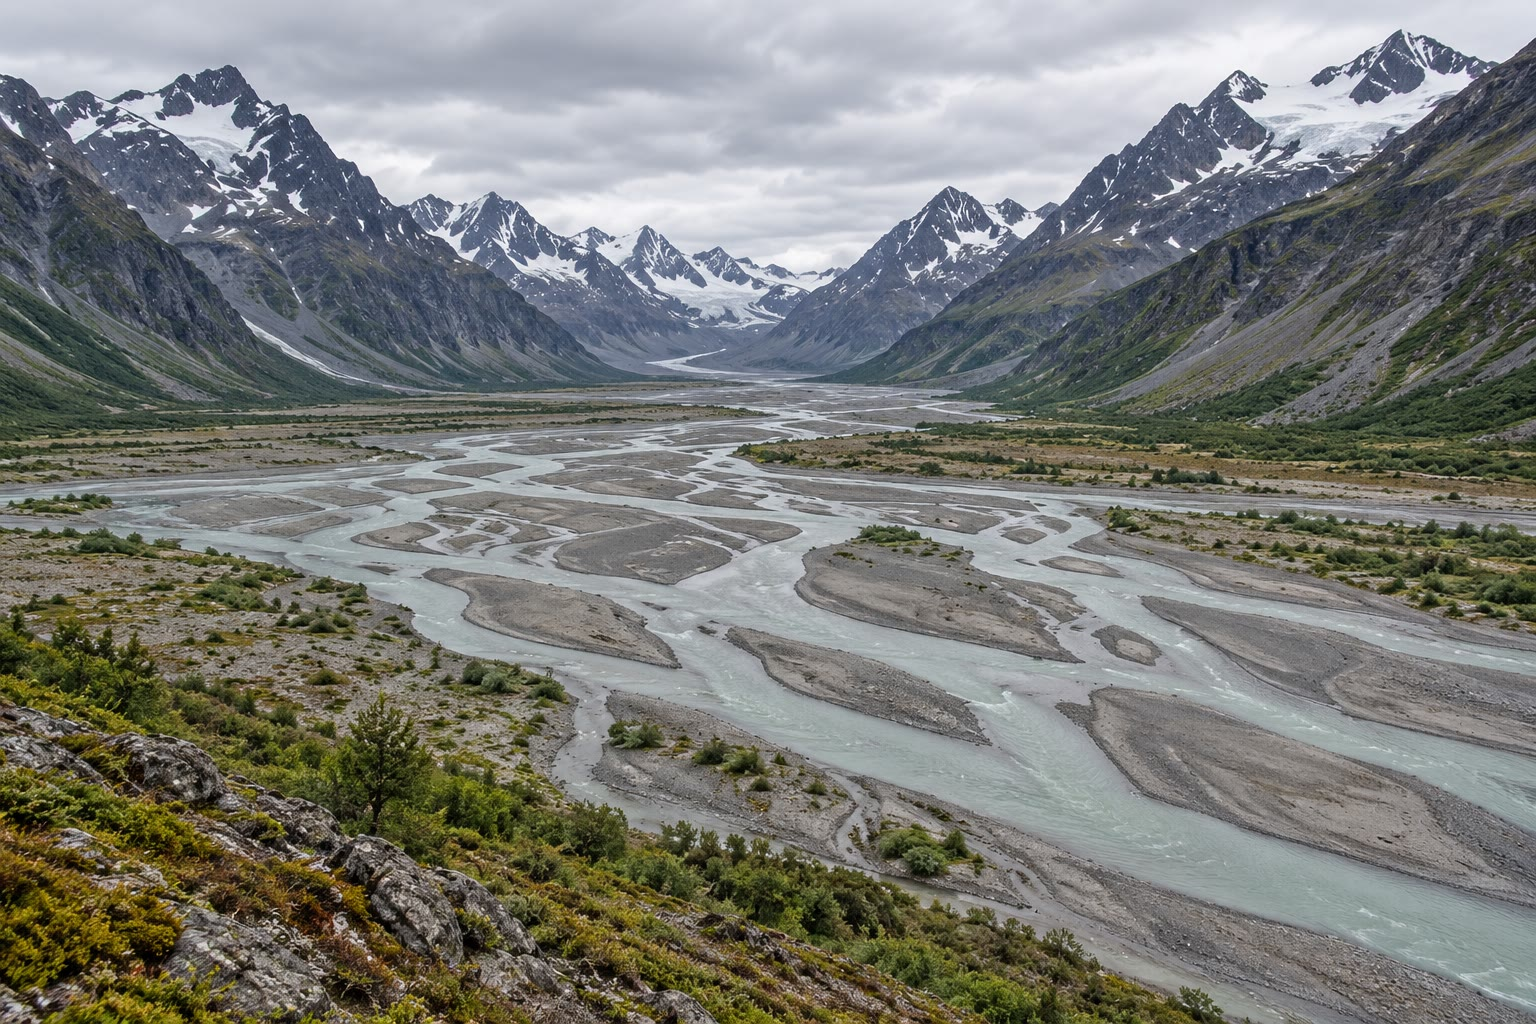
\includegraphics[width=0.66\linewidth]{images/book2/ai/g12-braided-river.jpg}

{\small 冰川山谷中的辫状河：浅水河道分岔
又汇合，夹在仅于洪水期才被水流搬动的砾石沙坝之间。
人工智能生成的插图。}
\end{omfigure}

测量河流所携带的物质，提供了求\omterm{def:g12:destruction-of-mountains:denudation}{剥蚀速率}的第二种方法。

\begin{method}[侵蚀收支]\label{met:g12:destruction-of-mountains:budget}
\begin{enumerate}
  \item 取河流一年内所携带沉积物的质量，并加上
        \omterm{def:g12:destruction-of-mountains:load}{溶解质}（若只知道固体部分，则将其除以
        $0.85$）。
  \item 除以岩石的密度（陆壳约为 \qty{2830}{kg/m^3}），
        以求得每年被移除的岩石体积。
  \item 除以\omterm{def:g10:drainage-basins:drainage-basin}{流域}面积：所得为每年被剥去的
        厚度。
  \item 乘以 $10^6$，以每百万年的米数表示。
\end{enumerate}
\end{method}
% ledger: earle:loads, cm95:crust

\begin{example}[密西西比河]\label{ex:g12:destruction-of-mountains:mississippi}
1900 年以前，密苏里–密西西比河水系每年向大海输送约
4 亿吨沉积物，\omterm{def:g10:drainage-basins:drainage-basin}{流域}面积约为 \qty{2980000}{km^2}。
计入\omterm{def:g12:destruction-of-mountains:load}{溶解质}后，$400/0.85 \approx 471$ 百万
吨，即每年约 $\num{4.71e11}/2830 \approx \qty{1.66e8}{m^3}$ 的岩石。
将其平摊于 $\qty{2.98e12}{m^2}$ 的面积上，得到的层厚为
\[
  \frac{\num{1.66e8}}{\num{2.98e12}} \approx \qty{5.6e-5}{m}
  \text{ 每年，约 } \qty{56}{m/Ma}.
\]
1987 年至 2006 年间，该河仅输送 1.45 亿吨沉积物，由此
可得约 \qty{20}{m/Ma}：1950 年代在密苏里河上修建的水坝
每年约截留 1 亿至 1.5 亿吨，其他工程截留的还要更多。
\end{example}
% ledger: mm10:mississippi, kammerer:mississippi, earle:loads, cm95:crust
% values: miss_before_1900_m_per_myr 55.8, miss_1987_2006_m_per_myr 20.2 (relief_decay.py)

同样的收支核算也可用于全球。人类改变河流之前，
河流每年向海岸输送约 155 亿吨固体沉积物；计入\omterm{def:g12:destruction-of-mountains:load}{溶解质}后，
约合每年 \qty{6.4}{km^3} 的岩石，
取自 \qty{1.48e8}{km^2} 的大陆：平均\omterm{def:g12:destruction-of-mountains:denudation}{剥蚀速率}
约为 \qty{43}{m/Ma}，接近铍-10
测量值的中位数。此后人类也改变了这两项：水土流失使
河流挟带的沉积物每年增加约 23 亿吨，而
超过 1000 亿吨沉积物如今积存于水坝之后。
% ledger: syvitski:modern-flux (Book 1 row, prehuman 15.5 Gt/yr with bed load), sy05:humans, data:etopo1 (land fraction 0.290, grade-11 hypsometry), cm95:crust
% values: world_volume_km3_per_yr 6.44, land_area_km2 1.48e8, world_m_per_myr 43.5 (relief_decay.py)

\section{从沉积物到岩石}

河流所携带的物质，在水流减缓之处沉积，包括山谷与
湖泊、三角洲，尤其是大陆
边缘的\omterm{def:g11:fossil-fuel-geology:basin}{沉积盆地}。沉积物一层层被掩埋，
并逐渐转变为岩石。

\begin{definition}[碎屑岩；成岩作用]\label{def:g12:destruction-of-mountains:diagenesis}
\emph{碎屑岩}\index{碎屑岩}是一种
由较老岩石与矿物的碎屑组成的沉积岩。
\emph{成岩作用}\index{成岩作用}是指将埋藏的沉积物
在较低温度下转变为岩石的一系列变化：\emph{压实}，
由\omterm{def:g11:fossil-fuel-geology:petroleum-system}{上覆岩层}的重量挤出孔隙中的水和空气；随后是\emph{置换沉淀}，
即孔隙水中结晶析出的矿物（方解石、石英、
赤铁矿、\omterm{def:g10:soil-formation:clay}{黏土矿物}）将颗粒胶结在一起。
\end{definition}
% ledger: earle:clastic

\omterm{def:g12:destruction-of-mountains:diagenesis}{碎屑岩}按碎屑的大小命名：
\begin{itemize}
  \item \textbf{砾岩}由圆状且粒径大于
        \qty{2}{mm} 的碎屑组成，\textbf{角砾岩}则由棱角状碎屑组成；
  \item \textbf{砂岩}由砂粒组成，颗粒粒径介于 \qty{2}{mm}
        与 \qty{0.063}{mm} 之间，多为石英，
        而石英是最能抵抗风化的矿物；
  \item \textbf{泥岩}中粉砂和黏土的含量至少为 \qty{75}{\percent}；
        若能沿薄层裂开，则为\textbf{页岩}。
\end{itemize}
% ledger: earle:clastic

\begin{omfigure}
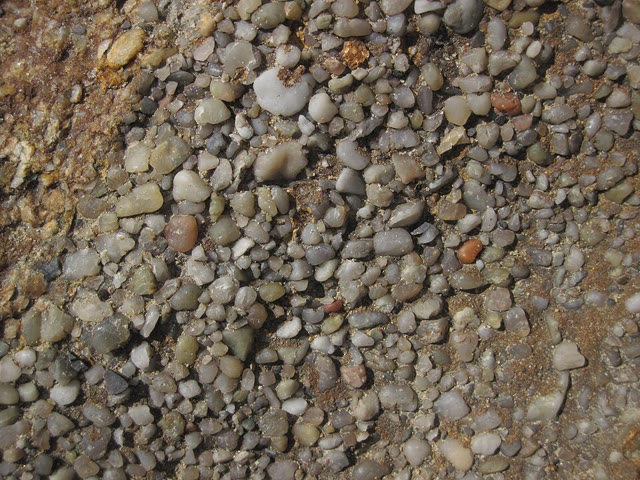
\includegraphics[width=0.5\linewidth]{images/book2/g12-stjohn-conglomerate.jpg}

{\small 来自俄亥俄州的石英卵石砾岩，属石炭纪：
圆状石英卵石，由较细的砂胶结而成。照片：James
St.~John (CC~BY~2.0)。}
\end{omfigure}
% ledger: photo:g12-conglomerate, ics:base.Carboniferous, ics:base.Permian (Lower Pennsylvanian lies in the Carboniferous)

碎屑记录了其搬运的经历。圆状卵石在河流
或海滩上滚动了很远，棱角状碎屑则几乎未经搬运。
几乎全由石英组成的砂岩，来自长期风化的岩石，
直到其他矿物都已风化为黏土。
% ledger: earle:clastic (rounded/angular, most sand grains quartz, the most resistant mineral)

\section{山根隆升}

若侵蚀只是从山脉顶部移走岩石，一座高 \qty{2}{km}
的山脉以 \qty{200}{m/Ma} 的速率被剥蚀，1000 万年后便会消失殆尽。
然而山脉漂浮于地幔之上。随着顶部岩石被移走，
岩柱变轻，并随之上升。

\begin{definition}[均衡回弹]\label{def:g12:destruction-of-mountains:rebound}
\emph{均衡回弹}\index{均衡回弹}是\omterm{def:g11:lithosphere-asthenosphere:lithosphere}{岩石圈}的某一区域
在荷载被移去时发生的上升——荷载可以是被侵蚀移走的岩石，
或融化的冰盖——直至恢复\omterm{def:g11:lithosphere-asthenosphere:isostasy}{地壳均衡}为止。
\end{definition}
% ledger: sella07:gia (rebound after ice unloading)

\begin{proposition}[侵蚀与回弹]\label{prop:g12:destruction-of-mountains:rebound}
在艾里模型中，当侵蚀从处于均衡状态的区域上移去厚度为 $e$ 的地壳，
该地壳密度为 $\rho_c$，地幔密度为 $\rho_m$，
则地表仅下降
\[
  \Delta h = e\left(1 - \frac{\rho_c}{\rho_m}\right),
\]
同时地壳底部上升 $e\,\rho_c/\rho_m$。
\end{proposition}

\begin{proof}
将顶部 $e$ 移去，地壳变薄 $e$。由艾里模型，
厚度减少 $e$ 的地壳，其高度降低 $e\,(\rho_m - \rho_c)/\rho_m = e(1 -
\rho_c/\rho_m)$。地壳顶部因此下降了这一量，其
厚度减少了 $e$，因此底部上升了 $e - e(1 -
\rho_c/\rho_m) = e\,\rho_c/\rho_m$。
\end{proof}

取 $\rho_c = \qty{2830}{kg/m^3}$，$\rho_m = \qty{3380}{kg/m^3}$，则 $1 -
\rho_c/\rho_m \approx 0.163$。移去 \qty{1}{km} 的岩石，地表仅降低
约 \qty{163}{m}：其余 \qty{837}{m} 由整个岩柱上升来补偿。
要使山脉降低 \qty{2000}{m}，侵蚀必须移去
约 $2000/0.163 \approx \qty{12300}{m}$ 的岩石。原本埋深超过
\qty{12}{km} 的岩石，即形成于山脉深部的变质岩和花岗岩，
出露地表：这正是古老、被剥蚀殆尽的造山带
大范围出露片岩、片麻岩和花岗岩的原因。
% ledger: cm95:crust, data:prem (rho 3.38 below the Moho)
% values: rebound_fraction 0.16272, lowering_per_km_m 162.7, root_rise_per_km_m 837.3, eroded_for_2000m_km 12.29 (relief_decay.py)

\begin{omfigure}
\begin{tikzpicture}[x=1cm, y=1cm, font=\scriptsize]
  % three columns: before, after erosion without rebound, after rebound
  \foreach \i/\top/\base/\lab in {0/3.0/-3.2/{处于均衡的山脉}, 1/2.0/-3.2/{侵蚀剥去 $e$}, 2/2.84/-2.36/{岩柱上升}} {
    \begin{scope}[xshift=\i*4.6cm]
      \fill[omLithPeridotite!45] (0,-3.6) rectangle (3.4,-0.6);
      \fill[omLithGranite!55, draw=black!60] (0.5,\base) -- (0.5,0) -- (1.0,\top) -- (2.4,\top) -- (2.9,0) -- (2.9,\base) -- cycle;
      \fill[omLithGranite!55, draw=black!60] (0,0) rectangle (0.5,-0.6);
      \fill[omLithGranite!55, draw=black!60] (2.9,0) rectangle (3.4,-0.6);
      \draw[black!40, densely dashed] (-0.1,0) -- (3.5,0);
      \node[anchor=north, align=center, text width=3.4cm] at (1.7,-3.75) {\lab};
    \end{scope}
  }
  % eroded slab, middle panel
  \draw[omThm, densely dashed] (4.6+1.0,3.0) -- (4.6+2.4,3.0);
  \draw[omThm, |-|] (4.6+2.65,3.0) -- node[right] {$e$} (4.6+2.65,2.0);
  % right panel: the old top and base
  \draw[omThm, densely dashed] (9.2+1.0,3.0) -- (9.2+2.4,3.0);
  \draw[omThm, densely dashed] (9.2+0.5,-3.2) -- (9.2+2.9,-3.2);
  \draw[-{Stealth}, omDef, line width=0.9pt] (9.2+1.7,-3.15) -- (9.2+1.7,-2.45);
  \node[omDef, anchor=west] at (9.2+3.0,-2.8) {山根上升};
  \node[anchor=west] at (9.2+3.0,2.95) {地表仅下降};
  \node[anchor=west] at (9.2+3.0,2.55) {仅 $0.16\,e$};
  \draw[black!60, |-|] (9.2+2.65,3.0) -- (9.2+2.65,2.84);
  % labels
  \node[anchor=west] at (3.45,-2.1) {地幔};
  \node at (1.7,-1.5) {地壳};
\end{tikzpicture}

{\small 侵蚀与\omterm{def:g12:destruction-of-mountains:rebound}{均衡回弹}（示意图，高度未按比例绘制）。左：
处于均衡状态的山脉及其\omterm{def:g12:continental-crust:root}{山根}。中：侵蚀从顶部移去厚度为 $e$ 的
岩层。右：变轻的岩柱上升，直至恢复\omterm{def:g11:lithosphere-asthenosphere:isostasy}{地壳均衡}；
地表最终仅比起始时低 $0.163\,e$，\omterm{def:g12:continental-crust:root}{山根}
已上升 $0.837\,e$。}
\end{omfigure}

同样的回弹今天仍可在荷载迅速消失的地方观测到。
末次盛冰期覆盖加拿大大部分地区的冰盖，
其最厚处位于哈德逊湾一带。该冰盖已融化，那里的陆地仍在
上升，据 GPS 测得约为每年 \qty{10}{mm}，即
\qty{10000}{m/Ma}，约为
\omterm{def:g10:drainage-basins:drainage-basin}{流域}平均\omterm{def:g12:destruction-of-mountains:denudation}{剥蚀速率}的五十倍。更靠南
越过五大湖，陆地以每年 1 至 \qty{2}{mm} 的速度下沉。
% ledger: sella07:gia, pb11:rates

\section{山脉能存在多久？}

\omterm{def:g10:drainage-basins:drainage-basin}{流域}越陡，侵蚀越快；对于大型\omterm{def:g10:drainage-basins:drainage-basin}{流域}，\omterm{def:g12:destruction-of-mountains:denudation}{剥蚀速率}
已被发现与其平均地形起伏成正比。下面取能体现这一规律的
最简单模型。

\begin{proposition}[山脉的指数衰减]\label{prop:g12:destruction-of-mountains:decay}
设 $h(t)$ 为山脉高出周围平原的平均海拔。若
\omterm{def:g12:destruction-of-mountains:denudation}{剥蚀速率}为 $E = k\,h$，$k$ 为常数，且\omterm{def:g11:lithosphere-asthenosphere:isostasy}{地壳均衡}
始终得以恢复，则
\[
  h(t) = h_0\, e^{-f k t}, \qquad f = 1 - \frac{\rho_c}{\rho_m},
\]
其中 $h_0$ 为 $t = 0$ 时的海拔。海拔每次除以 $e$ 所需的时间为
$\tau = 1/(fk)$，海拔减半所需时间为 $\tau \ln 2$。
\end{proposition}

\begin{proof}
在很短的时间 $\mathrm{d}t$ 内，侵蚀移去的厚度为 $E\,\mathrm{d}t
= k h\,\mathrm{d}t$，由前一命题，地表下降
了 $f k h\,\mathrm{d}t$。于是 $h' = -fk\,h$，此方程的
解为 $h(t) = h_0\,e^{-fkt}$。当 $t = \tau$ 时，$h = h_0/e$；
当 $h = h_0/2$ 时，$fkt = \ln 2$。
\end{proof}

对大型盆地的测量可得 $k$：若完全没有隆升，其地形起伏
将在约 1100 万年内降至十分之一。于是 $e^{-11k} = 0.1$，且 $k =
\ln 10/11 \approx 0.209$ 每百万年。无回弹（$f = 1$）时，
时间常数为 $1/k \approx 4.8$ 百万年。有回弹时，$f
\approx 0.163$，且
\[
  \tau = \frac{1}{0.163 \times 0.209} \approx 29 \text{ 百万年},
\]
而平均海拔每隔 $29 \ln 2 \approx 20$ 百万年减半：
回弹使山脉存在的时间延长约六倍。
% ledger: ahnert70:decay, cm95:crust, data:prem
% values: k_per_myr 0.20933, tau_none_myr 4.777, tau_rebound_myr 29.36, half_rebound_myr 20.35, half_none_myr 3.31 (relief_decay.py)

\begin{omfigure}
\begin{tikzpicture}
\begin{axis}[omrecord, width=0.7\linewidth, height=5.4cm, xmin=0, xmax=100, ymin=0, ymax=2100,
  xlabel={时间（百万年）}, ylabel={平均海拔（\unit{m}）},
  xtick={0,20,...,100}, ytick={0,500,...,2000}]
% computed in figdata/grade-12/relief_decay.py; ledger: ahnert70:decay, cm95:crust, data:prem
\addplot[omProp, line width=1.1pt, densely dashed] table[x=t_Myr, y=h_none] {figdata/out/grade-12-relief_decay-curve.dat};
\addplot[omDef, line width=1.1pt] table[x=t_Myr, y=h_rebound] {figdata/out/grade-12-relief_decay-curve.dat};
\draw[black!45, densely dotted] (axis cs:20.35,0) -- (axis cs:20.35,1000) -- (axis cs:0,1000);
\draw[omProp, line width=0.4pt] (axis cs:9,304) -- (axis cs:33,215);
\coordinate (none) at (axis cs:33.5,215);
\coordinate (reb) at (axis cs:45,780);
\end{axis}
\node[font=\scriptsize, text=omProp, anchor=west] at (none) {无回弹};
\node[font=\scriptsize, text=omDef, anchor=south west] at (reb) {有回弹};
\end{tikzpicture}

{\small 一座高 \qty{2000}{m} 的山脉，其平均海拔以与高度成比例的速率被剥蚀，
分别考虑有无\omterm{def:g12:destruction-of-mountains:rebound}{均衡回弹}的情形；有回弹时，
经过 20 百万年海拔减半（虚线）。
速率常数取自 Ahnert（1970）；地壳与
\omterm{def:g11:seismic-structure:moho}{莫霍面}以下地幔的密度。}
\end{omfigure}

阿巴拉契亚山脉可用来检验这一图景。其造山碰撞结束于二叠纪，
距今超过 2.5 亿年，约为模型使海拔减半所需时间的十二倍以上。
按模型计算，$2000 \times e^{-250/29} \approx
\qty{0.4}{m}$。然而，门奇尔山至今仍高出海平面 \qty{2037}{m}。
仅凭该模型无法解释现今的地形起伏：该地区此后必定再次隆升，
或其剥蚀速度比模型假设的更慢。
% ledger: usgs:alleghanian, usgs:alleghanian-age, ics:base.Triassic, ncparks:mitchell, ahnert70:decay
% values: h_after_250myr_rebound_m 0.40 (relief_decay.py)

因此山脉是循环的。自山脉剥蚀下来的岩石，最终堆积于\omterm{def:g11:fossil-fuel-geology:basin}{沉积盆地}，
在那里成为\omterm{def:g12:destruction-of-mountains:diagenesis}{碎屑岩}；其中部分岩石被埋藏得足够深，以致变质，甚至熔化，
部分经\omterm{def:g11:subduction-zones:subduction}{俯冲}作用进入地幔，
（见\cref{ch:g12:subduction-magmatism}），另有部分
在两\omterm{def:g12:mountain-building:collision}{大陆碰撞}时再次\omterm{def:g12:mountain-building:fold}{褶皱}，形成新的山脉。
% ledger: ss09:balance (sediment subducted), earle:collision (sediments of both margins in the mountains)

\begin{omfigure}
\begin{tikzpicture}
\begin{axis}[omsection, x=1.25cm, y=0.003125cm, xmin=0, xmax=9.49, ymin=-700, ymax=650,
  xlabel={距 A 点的距离（\unit{km}）}, ylabel={海拔（\unit{m}）},
  ytick={-600,-300,0,300,600}, tick label style={font=\scriptsize}, unbounded coords=jump]
% shared region tables (figdata/shared/region.py); unconformity from figdata/grade-12/relief_decay.py; ledger: region:name
\addplot[fill=black!8, draw=black!50, line width=0.3pt, even odd rule] table {figdata/out/shared-region-section-unit-schist.dat};
\addplot[fill=icsTriassic!20, draw=black!50, line width=0.3pt, even odd rule] table {figdata/out/shared-region-section-unit-sandstone.dat};
\addplot[fill=icsJurassic!25, draw=black!50, line width=0.3pt, even odd rule] table {figdata/out/shared-region-section-unit-limestone.dat};
\addplot[fill=icsJurassic!8, draw=black!50, line width=0.3pt, even odd rule] table {figdata/out/shared-region-section-unit-shale.dat};
\addplot[fill=icsCretaceous!20, draw=black!50, line width=0.3pt, even odd rule] table {figdata/out/shared-region-section-unit-chalk.dat};
\addplot[fill=omLithAlluv, draw=black!50, line width=0.3pt, even odd rule] table {figdata/out/shared-region-section-unit-alluvium.dat};
\addplot[black, line width=0.7pt] table {figdata/out/shared-region-section-ground.dat};
\addplot[omThm, line width=1.4pt] table[x=s_km, y=z_m] {figdata/out/grade-12-relief_decay-unconformity.dat};
\addplot[fault] table {figdata/out/shared-region-section-fault.dat};
\node[anchor=south east, font=\small\bfseries] at (axis cs:0,650) {A};
\node[anchor=south west, font=\small\bfseries] at (axis cs:9.49,650) {B};
\node[font=\scriptsize, fill=white, inner sep=1pt] at (axis cs:1.2,-520) {片岩，约 480 Ma};
\coordinate (unc) at (axis cs:1.6,-300);
\end{axis}
\node[font=\scriptsize, text=omThm, anchor=west, fill=white, inner sep=1pt] at ([xshift=4pt]unc) {不整合};
\end{tikzpicture}

\smallskip
{\small\tikz\fill[black!8, draw=black!50] (0,0) rectangle (0.35,0.22);~片岩 \quad
\tikz\fill[icsTriassic!20, draw=black!50] (0,0) rectangle (0.35,0.22);~砂岩（三叠纪） \quad
\tikz\fill[icsJurassic!25, draw=black!50] (0,0) rectangle (0.35,0.22);~石灰岩 \quad
\tikz\fill[icsJurassic!8, draw=black!50] (0,0) rectangle (0.35,0.22);~页岩 \quad
\tikz\fill[icsCretaceous!20, draw=black!50] (0,0) rectangle (0.35,0.22);~白垩 \quad
\omve{2.5}}

{\small 瓦尔登丘陵剖面 A--B，不整合以红色标出：
三叠纪砂岩铺设于片\omterm{def:g12:subduction-magmatism:batholith}{岩基}底之上的平坦底面，
此后经\omterm{def:g12:mountain-building:fold}{褶皱}与断裂。数据来自本系列对该区域的模型。}
\end{omfigure}
% values: unconformity sampled from region.contact_elevation('sandstone'); varden_gap_myr 58.1 (relief_decay.py)

瓦尔登丘陵保存了这样一次循环的记录。其基底为片岩，
片岩约 4.8 亿年前变质，其中侵入了花岗岩，
侵入时间约为 3.1 亿年前——两者都形成于古老造山带地表以下数千米深处。然而，
三叠纪砂岩约自 2.52 亿年前开始沉积，
直接覆盖在它们之上，界面平坦，即不整合。
在不到 6000 万年的时间里，那座古老山脉被剥蚀为平原，
其深部岩石被带至地表。随后，
海水漫过平原，将其掩埋。
% ledger: region:name (model: schist 480 Ma, granite 310 Ma, erosion, unconformity, Triassic cover), ics:base.Triassic
% values: varden_gap_myr 58.1 (relief_decay.py)

\section{练习}

\begin{exercise}[$\star$]\label{exo:g12:destruction-of-mountains:1}
写出下列各项对应的术语：（a）单位时间内从某一区域移去的岩石平均厚度；
（b）河流沿河床滚动和跳跃搬运的颗粒；（c）河流在溶液中搬运的
离子；（d）使埋藏的沉积物变为
岩石的各种变化；（e）移去荷载后\omterm{def:g11:lithosphere-asthenosphere:lithosphere}{岩石圈}的上升。
\end{exercise}

\begin{exercise}[$\star$]\label{exo:g12:destruction-of-mountains:2}
写出下列\omterm{def:g12:destruction-of-mountains:diagenesis}{碎屑岩}的名称：（1）由粒径为 \qtyrange{5}{20}{mm} 的圆形卵石
胶结而成的岩石；（2）粒径为 \qty{0.3}{mm} 的石英颗粒；（3）
粉砂和黏土占 \qty{90}{\percent}、能裂成\omterm{def:g11:minerals:thin-section}{薄片}的岩石；（4）棱角状
碎屑，粒径为 \qty{3}{cm}。
\end{exercise}

\begin{exercise}[$\star$]\label{exo:g12:destruction-of-mountains:3}
将下列速率换算为毫米/年：（1）\qty{54}{m/Ma}；（2）\qty{218}{m/Ma}；
（3）哈德逊湾附近每年 \qty{10}{mm} 的隆升，以 \unit{m/Ma} 计。
\end{exercise}

\begin{exercise}[$\star$]\label{exo:g12:destruction-of-mountains:4}
一条河流每年搬运 6000 万吨固体沉积物。估算其
\omterm{def:g12:destruction-of-mountains:load}{溶解质}负荷。已知\omterm{def:g12:destruction-of-mountains:load}{溶解质}平均占搬运总质量的
\qty{15}{\percent}。
\end{exercise}

\begin{exercise}[$\star$]\label{exo:g12:destruction-of-mountains:5}
将下列过程按由地表向下的顺序排列，说明花岗岩中一颗石英颗粒
所经历的变化：盆地沉积、花岗岩风化、被较年轻地层掩埋、
河流搬运、胶结。
\end{exercise}

\begin{exercise}[$\star\star$]\label{exo:g12:destruction-of-mountains:6}
水流由 \qty{30}{cm/s} 减慢至 \qty{5}{cm/s}。利用本章的数值，
说明河床上静止的 \qty{1}{mm} 沙粒
与已处于悬浮状态的 \qty{0.01}{mm} 粉砂颗粒，
在每一流速下各会发生什么变化。
\end{exercise}

\begin{exercise}[$\star\star$]\label{exo:g12:destruction-of-mountains:7}
一个面积为 \qty{50000}{km^2} 的盆地每年向海洋输送
400 万吨固体沉积物。试编制其侵蚀收支，计入\omterm{def:g12:destruction-of-mountains:load}{溶解质}，取 $\rho =
\qty{2830}{kg/m^3}$，并与铍-10 盆地侵蚀速率的中位数相比较。
\end{exercise}

\begin{exercise}[$\star\star$]\label{exo:g12:destruction-of-mountains:8}
（1）计算 $1 - \rho_c/\rho_m$，取 $\rho_c = \qty{2700}{kg/m^3}$ 且
$\rho_m = \qty{3300}{kg/m^3}$。（2）侵蚀掉
\qty{1}{km} 岩石后，地表会降低多少？（3）与本章的数值进行比较。
\end{exercise}

\begin{exercise}[$\star\star$]\label{exo:g12:destruction-of-mountains:9}
一块花岗岩约在山脉之下 \qty{8}{km} 深处结晶。（1）
侵蚀须移去多厚的岩石，才能使其出露地表？（2）
同时平均地表下降多少？（3）若速率为 \qty{200}{m/Ma}，
需要多长时间？
\end{exercise}

\begin{exercise}[$\star\star$]\label{exo:g12:destruction-of-mountains:10}
大陆的平均高程约为 \qty{794}{m}。（1）以
\qty{43}{m/Ma} 的速率，侵蚀移去同样厚度的岩层需要多长时间？
（2）若计入\omterm{def:g12:destruction-of-mountains:rebound}{均衡回弹}且速率保持不变，
需要多长时间？（3）为何大陆在
经过 40 亿年后仍高出海面？
\end{exercise}

\begin{exercise}[$\star\star$]\label{exo:g12:destruction-of-mountains:11}
超过 1000 亿吨沉积物堆积在大坝后方，这些大坝多
建于近五十年间。（1）取密度为
\qty{2830}{kg/m^3}，这些沉积物相当于多大体积的岩石？（2）以全球人类出现前的
每年 155 亿吨固体负荷计，这些沉积物相当于多少年的负荷？
\end{exercise}

\begin{exercise}[$\star\star\star$]\label{exo:g12:destruction-of-mountains:12}
证明：在本章的模型中，山脉的\omterm{def:g12:destruction-of-mountains:denudation}{剥蚀速率}为
$E(t) = k h_0 e^{-fkt}$。计算平均高程由 $h_0$ 降至 0 时
所移去的岩石总厚度，并用
\omterm{def:g12:destruction-of-mountains:rebound}{均衡回弹}命题解释该结果。
\end{exercise}

\begin{exercise}[$\star\star\star$]\label{exo:g12:destruction-of-mountains:13}
哈德逊湾附近陆地每年上升 \qty{10}{mm}。（1）若该速率
保持不变，经过 1000 年将上升多少？（2）此次上升是
冰盖融化后的回弹。取冰的密度为
\qty{900}{kg/m^3}，地幔密度取 \qty{3380}{kg/m^3}：在艾里模型中，
\qty{2}{km} 厚的冰融化后，陆地总共会上升多少？
（3）为何该速率会随时间减慢？
\end{exercise}
% ledger: sella07:gia, usgs:ice-density (ice about 90 % as dense as water), data:prem

\begin{exercise}[$\star\star\star$]\label{exo:g12:destruction-of-mountains:14}
密西西比河在 1900 年以前每年搬运 4 亿吨固体沉积物，
而在 1987--2006 年间每年为 1.45 亿吨。（1）计算其
两个时期\omterm{def:g10:drainage-basins:drainage-basin}{流域}的\omterm{def:g12:destruction-of-mountains:denudation}{剥蚀速率}，\omterm{def:g10:drainage-basins:drainage-basin}{流域}面积为 \qty{2980000}{km^2}，
并计入\omterm{def:g12:destruction-of-mountains:load}{溶解质}。（2）两者中哪一个更能反映
\omterm{def:g10:drainage-basins:drainage-basin}{流域}的自然侵蚀？（3）大坝每年截留 1 亿至 1.5 亿吨，
这能否解释全部的减少量？
\end{exercise}

\begin{exercise}[$\star\star\star$]\label{exo:g12:destruction-of-mountains:15}
在瓦尔登丘陵，约 3.1 亿年前侵入的一块花岗岩位于
三叠纪砂岩之下，该砂岩约自 2.52 亿年前开始沉积。
设该花岗岩在地下 \qty{6}{km} 深处结晶。（1）其上方至少被移去了
多厚的岩石？（2）这至少需要多大的平均\omterm{def:g12:destruction-of-mountains:denudation}{剥蚀速率}？
（3）与各盆地的实测速率进行比较。
\end{exercise}

\begin{problem}[{周末问题——夷平一座山脉需要多长时间？}]
\label{pb:g12:destruction-of-mountains:1}
% ledger: pb11:rates, ahnert70:decay, cm95:crust, data:prem, usgs:alleghanian, usgs:alleghanian-age, ics:base.Triassic, ncparks:mitchell, photo:g12-appalachians
% values (relief_decay.py): k 0.20933/Myr, E0 418.7 m/Myr, f 0.16272, tau 4.777 / 29.36 Myr, half-lives 3.31 / 20.35 Myr
一座年轻山脉的平均高程比周围的平原高出
\qty{2000}{m}。其河流以与高度成正比的速率侵蚀山体，即 $E = kh$，
其中 $k = 0.209$（单位：每百万年）。地壳密度为
\qty{2830}{kg/m^3}，其下地幔密度为 \qty{3380}{kg/m^3}。

\medskip
\noindent\textbf{第一部分——侵蚀速率。}
\begin{enumerate}
  \item 计算该山脉当前的\omterm{def:g12:destruction-of-mountains:denudation}{剥蚀速率}，单位为 \unit{m/Ma}。
  \item 将其换算为毫米/年。
  \item 将其与地震活动盆地实测的平均速率
        （\qty{367}{m/Ma}）及安静盆地的（\qty{182}{m/Ma}）相比较。
  \item 盆地的哪一特征最能预测其侵蚀速率？
  \item 该山脉每平方千米每年有多少吨岩石
        离开该区域？
\end{enumerate}

\medskip
\noindent\textbf{第二部分——无回弹。}
\begin{enumerate}[resume]
  \item 若速率保持当前值，将
        \qty{2000}{m} 岩石全部移去需要多长时间？
  \item 事实上，山脉被降低时速率随之下降。写出方程
        $h' = -kh$ 及其在 $h(0) = \qty{2000}{m}$ 下的解。
  \item 时间常数 $1/k$ 是多少？
  \item 海拔降至一半需要多长时间？
  \item 验证经过 1100 万年后，海拔仍剩下十分之一。
\end{enumerate}

\medskip
\noindent\textbf{第三部分——有回弹。}
\begin{enumerate}[resume]
  \item 计算 $f = 1 - \rho_c/\rho_m$。
  \item 当侵蚀掉 \qty{100}{m} 岩石时，地表下降多少，
        而根部上升多少？
  \item 写出 $h$ 的新方程及其解。
  \item 要使山脉从
        \qty{2000}{m} 降至 \qty{200}{m}，需要侵蚀掉多厚的岩石？
  \item 这会使哪些类型的岩石出露到地表？
\end{enumerate}

\medskip
\noindent\textbf{第四部分——时间常数。}
\begin{enumerate}[resume]
  \item 计算有回弹情形下的时间常数。
  \item 山脉降至其高度的十分之一需要多长时间？
  \item 经过 2 亿年后，它有多高？
  \item 阿巴拉契亚造山运动结束于 2.5 亿多年前。
        若该山脉此后再未被抬升，模型给出的
        2.5 亿年后的高度是多少？米奇尔山目前仍高出海平面 \qty{2037}{m}，
        这说明了什么？
  \item 总结：山脉的平均海拔
        需要多少百万年才能减半？
\end{enumerate}
\end{problem}
